% Options for packages loaded elsewhere
\PassOptionsToPackage{unicode}{hyperref}
\PassOptionsToPackage{hyphens}{url}
%
\documentclass[
  english,
  man,floatsintext]{apa6}
\usepackage{lmodern}
\usepackage{amssymb,amsmath}
\usepackage{ifxetex,ifluatex}
\ifnum 0\ifxetex 1\fi\ifluatex 1\fi=0 % if pdftex
  \usepackage[T1]{fontenc}
  \usepackage[utf8]{inputenc}
  \usepackage{textcomp} % provide euro and other symbols
\else % if luatex or xetex
  \usepackage{unicode-math}
  \defaultfontfeatures{Scale=MatchLowercase}
  \defaultfontfeatures[\rmfamily]{Ligatures=TeX,Scale=1}
\fi
% Use upquote if available, for straight quotes in verbatim environments
\IfFileExists{upquote.sty}{\usepackage{upquote}}{}
\IfFileExists{microtype.sty}{% use microtype if available
  \usepackage[]{microtype}
  \UseMicrotypeSet[protrusion]{basicmath} % disable protrusion for tt fonts
}{}
\makeatletter
\@ifundefined{KOMAClassName}{% if non-KOMA class
  \IfFileExists{parskip.sty}{%
    \usepackage{parskip}
  }{% else
    \setlength{\parindent}{0pt}
    \setlength{\parskip}{6pt plus 2pt minus 1pt}}
}{% if KOMA class
  \KOMAoptions{parskip=half}}
\makeatother
\usepackage{xcolor}
\IfFileExists{xurl.sty}{\usepackage{xurl}}{} % add URL line breaks if available
\IfFileExists{bookmark.sty}{\usepackage{bookmark}}{\usepackage{hyperref}}
\hypersetup{
  pdftitle={Assessing sampling methods for generalization from RCTs: Modeling recruitment and participation},
  pdfauthor={Gleb Furman1 \& James E. Pustejovsky2},
  pdflang={en-EN},
  pdfkeywords={generalizability, sampling, MRT},
  hidelinks,
  pdfcreator={LaTeX via pandoc}}
\urlstyle{same} % disable monospaced font for URLs
\usepackage{graphicx,grffile}
\makeatletter
\def\maxwidth{\ifdim\Gin@nat@width>\linewidth\linewidth\else\Gin@nat@width\fi}
\def\maxheight{\ifdim\Gin@nat@height>\textheight\textheight\else\Gin@nat@height\fi}
\makeatother
% Scale images if necessary, so that they will not overflow the page
% margins by default, and it is still possible to overwrite the defaults
% using explicit options in \includegraphics[width, height, ...]{}
\setkeys{Gin}{width=\maxwidth,height=\maxheight,keepaspectratio}
% Set default figure placement to htbp
\makeatletter
\def\fps@figure{htbp}
\makeatother
\setlength{\emergencystretch}{3em} % prevent overfull lines
\providecommand{\tightlist}{%
  \setlength{\itemsep}{0pt}\setlength{\parskip}{0pt}}
\setcounter{secnumdepth}{-\maxdimen} % remove section numbering
% Make \paragraph and \subparagraph free-standing
\ifx\paragraph\undefined\else
  \let\oldparagraph\paragraph
  \renewcommand{\paragraph}[1]{\oldparagraph{#1}\mbox{}}
\fi
\ifx\subparagraph\undefined\else
  \let\oldsubparagraph\subparagraph
  \renewcommand{\subparagraph}[1]{\oldsubparagraph{#1}\mbox{}}
\fi
% Manuscript styling
\usepackage{upgreek}
\captionsetup{font=singlespacing,justification=justified}

% Table formatting
\usepackage{longtable}
\usepackage{lscape}
% \usepackage[counterclockwise]{rotating}   % Landscape page setup for large tables
\usepackage{multirow}		% Table styling
\usepackage{tabularx}		% Control Column width
\usepackage[flushleft]{threeparttable}	% Allows for three part tables with a specified notes section
\usepackage{threeparttablex}            % Lets threeparttable work with longtable

% Create new environments so endfloat can handle them
% \newenvironment{ltable}
%   {\begin{landscape}\begin{center}\begin{threeparttable}}
%   {\end{threeparttable}\end{center}\end{landscape}}
\newenvironment{lltable}{\begin{landscape}\begin{center}\begin{ThreePartTable}}{\end{ThreePartTable}\end{center}\end{landscape}}

% Enables adjusting longtable caption width to table width
% Solution found at http://golatex.de/longtable-mit-caption-so-breit-wie-die-tabelle-t15767.html
\makeatletter
\newcommand\LastLTentrywidth{1em}
\newlength\longtablewidth
\setlength{\longtablewidth}{1in}
\newcommand{\getlongtablewidth}{\begingroup \ifcsname LT@\roman{LT@tables}\endcsname \global\longtablewidth=0pt \renewcommand{\LT@entry}[2]{\global\advance\longtablewidth by ##2\relax\gdef\LastLTentrywidth{##2}}\@nameuse{LT@\roman{LT@tables}} \fi \endgroup}

% \setlength{\parindent}{0.5in}
% \setlength{\parskip}{0pt plus 0pt minus 0pt}

% \usepackage{etoolbox}
\makeatletter
\patchcmd{\HyOrg@maketitle}
  {\section{\normalfont\normalsize\abstractname}}
  {\section*{\normalfont\normalsize\abstractname}}
  {}{\typeout{Failed to patch abstract.}}
\patchcmd{\HyOrg@maketitle}
  {\section{\protect\normalfont{\@title}}}
  {\section*{\protect\normalfont{\@title}}}
  {}{\typeout{Failed to patch title.}}
\makeatother
\shorttitle{Assessing sampling methods for generalization from RCTs}
\keywords{generalizability, sampling, MRT}
\usepackage{csquotes}
\usepackage{rotating}
\usepackage{float}
\geometry{twoside=false, top=1in, bottom=1in, left=1in, right=1.15in}
\usepackage[textwidth=1in, textsize=tiny]{todonotes}
\raggedbottom
\newcommand{\JEP}[1]{\todo[color=blue!20]{#1}}
\newcommand{\GF}[1]{\todo[color=orange]{#1}}
\ifxetex
  % Load polyglossia as late as possible: uses bidi with RTL langages (e.g. Hebrew, Arabic)
  \usepackage{polyglossia}
  \setmainlanguage[]{english}
\else
  \usepackage[shorthands=off,main=english]{babel}
\fi

\title{Assessing sampling methods for generalization from RCTs: Modeling recruitment and participation}
\author{Gleb Furman\textsuperscript{1} \& James E. Pustejovsky\textsuperscript{2}}
\date{}


\affiliation{\vspace{0.5cm}\textsuperscript{1} University of Texas at Austin\\\textsuperscript{2} University of Wisconsin-Madison}

\abstract{
Educational research aimed at informing policy decisions should ideally be robustly designed to detect causal effects at the population level. Large scale, multi-site randomized trials often rely on vague convenience sampling methodology when recruiting districts and schools, resulting in relatively homogeneous samples that may differ greatly from the intended population of interest. Retrospective methods that quantify and statistically adjust for those differences are promising but may have difficulty overcoming substantial selection bias. Designing sampling methods that focus on generalizability may be a more effective, albeit costly, solution. However, there is a lack of methodological research examining the effectiveness of such strategies in education research contexts. We propose a framework for conducting such research based on formal models for study recruitment and participation. Using this framework, we then examine one promising method, stratified balanced sampling (SBS), in the context of recruiting a representative sample of schools for a large trial. Using simulations based on real sampling frames, we compare SBS to stratified and unstratified versions of convenience sampling and probability sampling. Under our modeling assumptions, we find that SBS and stratified random sampling result in highly generalizable samples. These methods are extremely costly to implement, however, especially when the population average willingness to participate is low. Stratified convenience sampling represents a potential compromise.\JEP{One more sentence about future research needs.}
}



\begin{document}
\maketitle

\hypertarget{introduction}{%
\section{Introduction}\label{introduction}}

The multi-site randomized trial (MRT) has become a common design for evaluating the effectiveness of educational interventions. An MRT is a randomized control trial that takes place across multiple distinct sites, such as school districts, medical clinics, or geographic areas, with random assignment taking place either at the site or unit level. In education research, an MRT might entail recruiting multiple schools in each of several districts. Once a sample of schools is recruited, students, classes, teachers, or whole schools are randomly assigned either to receive an intervention (treatment group) or to an alternative conditions, such as continuing business-as-usual (control group).

Well-executed MRTs with low attrition support a high level of internal validity, in that we can be confident that observed differences in outcomes between the treatment and control groups represent causal effects of treatment assignment. One might also expect that running a trial across multiple sites would support a high level of external validity, or generalizability, because it provides a basis for detecting and investigating cross-site variation in treatment effects (Raudenbush \& Bloom, 2015).
Ostensibly, this features allows researchers to generalize findings to a larger population than estimates from a single-site design (Raudenbush \& Liu, 2000). However, such claims rest on strong and rather ambiguous assumptions about the goal of generalization.

In the context of intervention studies, generalizability describes how well the effect of an intervention would hold for units outside of the study.
For instance, results of a randomized trial are often interpreted as estimates of the sample average treatment effect (SATE), or the average effect of intervention for the set of units that actually participated in the study (Gerber \& Green, 2012).
If the study sample is representative of a larger population, a SATE estimate can also be interpreted as a reasonable estimate of the average effect of intervention within the larger population of units, or population average treatment effect (PATE), without any additional adjustments. However, if the sample is compositionally different from the population of interest, and if response to intervention varies across units or sites in the population, then the SATE no longer provides an unbiased estimate of the PATE.\todo[color=blue!20]{Cites supporting this?}

Several studies have found that schools and districts that participate in large scale randomized trials differ substantially from the national population and from policy-relevant sub-populations (Fellers, 2017; Stuart, Bell, Ebnesajjad, Olsen, \& Orr, 2017).\todo[color=blue!20]{Update with recent refs}
This suggests that current research practices yield non-representative samples.
In turn, non-representative samples may lead to substantially biased estimates of population-level effects (Olsen, Orr, Bell, \& Stuart, 2013; Shadish, Cook, \& Campbell, 2002). Beyond accurate effects estimates, generalizability can also be a question of equity. For instance, small under-served rural districts are underrepresented in RCTs sponsored by Institute of Education Sciences (Fellers, 2017; Stuart et al., 2017), and thus may be less likely to benefit from federally funded education research.

One way to achieve strong generalizability is to select sites from a well-defined population with known probabilities of selection. Assuming random assignment with full compliance and low attrition, this design enables unbiased estimation of the SATE. Using the known sampling probabilities, the SATE can then be adjusted to estimate the PATE. Unfortunately, probability sampling is rarely used in large-scale impact evaluations (Olsen et al., 2013; Shadish et al., 2002). Instead, researchers often opt for convenience or purposive sampling. These methods are much less expensive to implement, but are not usually designed to achieve population representation.

\hypertarget{retrospective-generalization-methods}{%
\subsection{Retrospective generalization methods}\label{retrospective-generalization-methods}}

A growing body of methodological research has considered how to estimate PATEs from non-representative samples using retrospective propensity score analysis (Kern, Stuart, Hill, \& Green, 2016; O'Muircheartaigh \& Hedges, 2014; Stuart, Cole, Bradshaw, \& Leaf, 2011; Tipton, 2013a).
In order to justify a claim of generalizabilty, these methods rely on the availability of data for a clearly specified inference population.
The data must include covariates that predict treatment effect heterogeneity.
The methods then work by re-weighting the sample (or otherwise adjusting) to generate estimates of the PATE.
A shortcoming of retrospective generalization methods is under-coverage (Groves, 2004) which occurs when a sample lacks units corresponding to a sub-group of the inference population. Under-coverage can be assessed using several techniques that identify how well a sample would generalize to a specific population (Stuart et al., 2011; Tipton, 2014). If under-coverage is great enough to prevent use of statistical adjustment for estimating the PATE, then the inference population must be redefined. However, re-defining the inference population diminish the relevance of study results, undermining the substantial investment into large-scale MRTs.

\hypertarget{stratified-balanced-sampling}{%
\subsection{Stratified balanced sampling}\label{stratified-balanced-sampling}}

A series of recent papers instead advocate designing robust sampling methods that focus on generalizability at the recruitment stage (Tipton, 2013a, 2013b). Like retrospective adjustment, these methods also require a well-defined and enumerated population for which there is extant data, making them especially relevant in the educational context.\todo[color=blue!20]{Weird way to bring this point up. Move closer to top?}
One method in particular, Stratified Balanced Sampling (SBS), has received attention from intervention effectiveness researchers due to its accessibility.

SBS involves using cluster analysis to split the population into smaller, more homogeneous strata. Sites within each stratum are then ranked according to how well they represent the stratum and highly representative sites are prioritized for recruitment.
Researchers who are interested in using this to sample schools may even use a website (www.thegeneralizer.org) that guides them through this process using data from the Common Core of Data.
Several studies have described potential theoretical benefits of SBS (Tipton, 2013b; Tipton et al., 2016). First, SBS requires that researchers specify the inference population and justify targeting specific sites. Thus, it enforces a degree of clarity regarding the goal of generalization, which has often been lacking even in large-scale MRTs in education (Tipton, Spybrook, Fitzgerald, Wang, \& Davidson, 2020). Second, SBS should theoretically improve sample representation and reduce under-coverage, thereby improving generalization to the specified target population. Further, SBS easily integrates with retrospective statistical adjustment techniques. Even if balance is only partially improved at the sampling stage, coverage errors will still be reduced, mitigating the need to redefine the inference population post-hoc.
Finally, SBS requires researchers to carefully document the recruitment process, which supports transparency and enables more rigorous critique of the sampling design and study inferences, as well as enabling follow-up analysis on participation behavior such as systematic differences between participants and non-responders.

There are, of course, several limitations as well. SBS depends on the existence of a rich set of observed covariates related to treatment heterogeneity and sample selection for each site in the population. Most readily available extant data primarily consist of demographics and may not contain information on covariates that are more proximally related to variation in treatment effect, which can result in omitted variable bias (Tipton, 2013b). Additionally, SBS requires more resources to implement than a simple convenience sample. Recruiting ranked sites from multiple strata requires a coordinated effort between recruiters (Tipton, Hallberg, Hedges, \& Chan, 2017). This means that recruiters cannot work independently and must rely on a partnership with researchers implementing this method.

At least one research group has implemented SBS in a large-scale multi-site educational intervention study and documented their experiences (Tipton \& Matlen, 2019). The authors reported success in selecting a highly generalizable sample, but substantial efforts were required to develop the sample frame, generate optimal strata, and coordinate with recruiters.
This was compounded by the unavailability of data necessary for identifying the sampling frame.
Additionally, though the recruiters reported that working within the strata did not burden their efforts, certain strata were more difficult to recruit from than others.
These findings raise an important and pragmatic question: do the advantages of SBS justify the additional resources necessary to implement it?
And how do other methods of sample recruitment compare in terms of their ability to obtain representative samples and their cost to implement?

\hypertarget{aims}{%
\subsection{Aims}\label{aims}}

In order for researchers to make informed decisions about sampling strategies, there is a need to better understand both the performance and the cost of SBS, relative to other sample recruitment methods.
The goal of the current paper is to describe a framework for making such assessments and to demonstrate how it can be applied.
Central to our proposed framework is that sample representation is influenced by two distinct processes: the researcher's recruitment method and schools' participation decisions.
The recruitment method influences whether a population unit is approached by researchers, and includes methods such as SBS, probability sampling, and convenience sampling.
Because convenience sampling can take many forms in practice, we put forth a simple model, which prioritizes sites that are more likely to agree to participate.
To model school district participation decisions, we use extant demographic data and reported characteristics of schools that have been recruited to large-scale trials to simulate a participation propensity score.

After describing formal models for recruitment and participation, we report a simulation study comparing the performance and feasibility of the sampling methods. We conceptualize generalizability in terms of whether obtained samples are similar to the target population on observable site characteristics. We conceptualize
feasibility in terms of researcher recruitment effort to obtain a target sample size and how sample participation is distributed across the population.
As with many simulation studies, findings from those reported below are tentative and limited due to some of the simplifying assumptions that we impose--particularly assumptions about the school participation model and the process of convenience sampling.
Despite these assumptions, we argue that the simulations nonetheless provide insights into the relative performance of different recruitment methods.
Moreover, the limitations of the simulations highlight the need for more and better empirical data about recruitment efforts, so that key assumptions of the framework can be further refined.

The remainder of the paper is organized as follows. In the next section, we describe the framework for assessing recruitment methods by proposing a model for school participation decisions and several models for sample recruitment, including SBS and other sampling methods. In the following section, we provide an illustration of using cluster analysis to define population strata---the critical initial step in SBS, and one that may have broader utility as well. We then demonstrate how to implement our proposed framework in a simulation, in which we assess the relative performance of SBS and other recruitment methods. In the final two sections, we report the simulation results and discuss limitations and directions for future research in this area.

\hypertarget{methods-and-models}{%
\section{Methods and Models}\label{methods-and-models}}

The goal of recruitment is to obtain a study sample that is compositionally similar to a population of interest, such that treatment effects detected in the study can be generalized to that population.
Ideally, we would like to obtain a sample that is similar to the population on any and all covariates that are associated with treatment effect heterogeneity.
However, both SBS and retrospective generalization methods aim toward a more limited goal of obtaining a sample that is similar to the population on a set of measured covariates.\todo[color=blue!20]{More discussion of what these covariates should be}
We follow this conceptualization of generalizability.

Formally, we shall consider a population of \(N\) units (such as schools), indexed by \(j = 1,...,N\).
We assume that we have a dataset containing \(P\) covariates, \(\mathbf{x}_j = \left(x_{1j},...,x_{Pj}\right)\), for every unit in the population. The covariates may be a mixture of continuous, binary, and categorical data.
Following Tipton (2013b), we assume that the researcher's goal is to select a sample of \(n\) sites such that there is balance along \(\mathbf{x}_j\) between the sample and the population, indicating that the population is compositionally represented by the sample.
We measure balance using the standardized mean difference (\(SMD\)) between the sample and population for a given covariate. For covariate \(p\), the SMD is calculated as
\begin{align} \label{eq:SMD}
SMD_p = \frac{\bar{x}_p - \mu_p}{\sigma_p}
\end{align}
where \(\bar{x}_p\) is the sample mean of covariate \(p\), \(\mu_p\) is the covariate mean in the population, and \(\sigma_p\) is the standard deviation of the covariate in the population. \(SMD\) values closer to zero indicate greater balance between the sample and the population.\todo[color=blue!20]{More discussion of how to interpret balance across the set of $P$ covariates.}

When recruiting a sample, selection bias, or imbalance between the sample and the population, can arise from at least two distinct processes: recruitment methods and the decisions of individual units about whether to participate. Our goal is to assess the effectiveness and costs of different recruitment methods, such as SBS, probability sampling, and convenience sampling. However, any of the recruitment methods must contend with unit non-response, such as when school leaders decline to participate in the research study.
Our proposed framework treats the two processes as distinct, allowing us to isolate the influence of different recruitment methods.

\hypertarget{modeling-selection-bias}{%
\subsection{Modeling Selection Bias}\label{modeling-selection-bias}}

Selection bias stems from two sources: (1) unit participation decisions (self-selection) and (2) researcher sampling behavior (recruitment bias). To model the former we propose a simple participation propensity score. Let \(E_j\) be a binary indicator of \emph{potential participation}---that is, whether a school would participate in the study \emph{if approached for recruitment}, where \(E_j = 1\) if the school would agree and \(E_j = 0\) if the school would refuse. Let \(\pi_j\) represent the participation propensity score, or the probability that unit \(j\) would agree to participate in an RCT if approached. We will model \(\pi_j\) using a basic logistic regression, where:
\begin{align} 
\label{eq:RGM}
\log\left(\frac{\pi_j}{1 - \pi_j}\right) = \beta_0 + \mathbf{x}_j \boldsymbol\beta
\end{align}
where \(\mathbf{x}_j\) is an \(1\times P\) vector of covariates that predict sample selection for each unit, and \(\boldsymbol\beta\) is a vector of coefficients associated with those covariates. Participation for unit \(j\) is then determined by sampling from a Bernoulli distribution with probability equal to \(\pi_j\):
\begin{equation}
\label{eq:Ej}
E_j \sim B(\pi_j).
\end{equation}
In this manner, \(\pi_j\) is a constant school characteristic, whereas \(E_j\) can vary across replications of the sampling process.
\todo[color=blue!20]{Discuss assumptions behind this model.}\todo[color=blue!20]{Discuss difficulty of estimating this model from extant data, due to non-representative samples. Also how will we develop assumptions about values of $\boldsymbol\beta$?}

\hypertarget{sampling-methods}{%
\subsection{Sampling Methods}\label{sampling-methods}}

In the remainder of this section, we propose formal models for several sampling procedures. The scope of procedures that we review here is not meant to be comprehensive. However, by formalizing them in this fashion we hope to make the procedures transparent, reproducible, and modifiable to easily fit other circumstances which may be of interest for study.

For each method, we model the sampling process as observing the potential participation indicator for schools in a ranked list, where the order in which schools are contacted is determined by a score \(S = S_1,...,S_N\). Different sampling procedures are defined by different methods of determining the scores. Let \(Z_j(S)\) be an indicator whether school \(i\) is sampled based on the score \(S\).
For the un-stratified sampling methods, we determined \(Z_1(S),...,Z_N(S)\) by sorting schools according to \(S\) and selecting the first \(n\) schools with \(E_j = 1\).
Specifically,
\begin{equation}
\label{eq:Zj}
Z_j(S) = I\left[n \geq \sum_{i=1}^N E_i I\left(S_i \leq S_j\right)\right]
\end{equation}
where \(I(C)\) denotes the indicator function, equal to 1 if \(C\) is true and otherwise equal to 0. Based on the sample selection indicators, we calculate the number of schools contacted as
\begin{equation}
\label{eq:R}
R(S) = \max \{S_1 Z_1, S_2 Z_2, ..., S_N Z_N\}.
\end{equation}

Several of the sampling methods that we shall consider involve use of stratification. For these methods, we will assume that the population is divided into a set of \(K\) strata and that the target sample size for each stratum is based on proportional allocation.\todo[color=blue!20]{Justify proportional allocation}
Letting \(N_k\) denote the total number of schools in stratum \(k\), we set a target sample size of \(n_k = [n \times N_k / N]\) for stratum \(k = 1,...,K\), where \([x]\) is the integer nearest to \(x\).
Let \(G_j \in \{1,...,K\}\) be the stratum assignment of unit \(j\), for \(j = 1,...,N\).
For the stratified sampling methods, the process for determining participation is applied separately within each stratum, so that
\begin{equation}
\label{eq:Zj-strat}
Z_j(S) = I\left[n^{G_j} \geq \sum_{i=1}^N E_i I\left(S_i \leq S_j, G_i = G_j\right)\right]
\end{equation}
and
\begin{equation}
\label{eq:R-strat}
R_k(S) = \max \{S_1 Z_1 I(G_1=k) , S_2 Z_2 I(G_2=k), ..., S_N Z_N I(G_N=k)\},
\end{equation}
with \(R(S) = \sum_{k=1}^K R_k(S)\).

\hypertarget{random-sampling}{%
\subsection{Random Sampling}\label{random-sampling}}

As previously mentioned, unstratified random sampling (URS) is typically highly impractical in the context of educational MRTs. However, URS is nonetheless interesting as a theoretically simple ideal against which to compare other sampling methods. We can simulate URS sampling by ranking each school according to a random number from a uniform distribution, so that their order of recruitment is determined by the score \(S_j \sim U(0, 1)\).

In practice, methods such as cluster sampling, stratified sampling, or a combination of both would likely offer advantages over unstratified random sampling. We therefore also simulate a stratified random sample (SRS), with strata determined by the results of the cluster analysis and using a proportional allocation.

\hypertarget{convenience-sampling}{%
\subsection{Convenience Sampling}\label{convenience-sampling}}

Modeling recruitment bias is less straightforward. Self-selection is present as long as sites have the ability to choose whether or not to participate. On the other hand, recruitment bias depends on whatever strategy is used for selecting sites in the first place. It can be avoided all together by using probability sampling techniques, where the probability that a site will be invited to participate is known and can be accounted for in the outcome analysis. However, this is not often feasible in the case of large-scale MRTs. Subsets of schools are likely to be overlooked if samples are too small, or when participation rates are too low. Further, random sampling from a broad population (such as an entire country) is likely to produce samples that are geographically dispersed, creating logistic difficulties for data collection and treatment implementation. As a result, researchers often eschew probability sampling in favor of convenience sampling (Gerber \& Green, 2012; Shadish et al., 2002).

Since researchers rarely operationalize and report their process for selecting a convenience sample, the question of what drives recruitment bias, and how to model it, is left largely open-ended. As a first step, we will entertain the strong assumption that the purpose of convenience sampling is to minimize effort. If we further assume that recruiters have some prior knowledge of how likely schools are to participate if approached, then we can model this selection mechanism as recruiters prioritizing schools with a higher propensity to participate. We refer to this as the \enquote{low hanging fruit} approach to convenience sampling.

We also simulate two convenience sampling methods: unstratified (UCS) and stratified convenience sampling (SCS). Here, we assume that recruiters have some knowledge of each schools' probability of participating, if approached, and that they prioritize higher probability schools in order to minimize effort. To operationalize unstratified convenience sampling, we assume that schools are approached for recruitment one at a time, with their order determined by sampling without replacement, and with probability proportional to participation propensity scores \(\pi^P_1,...,\pi^P_N\).
Once a school is selected and assigned a rank, the next school is selected with a probability proportional to the weights of the remaining schools. Once all ranks are assigned, schools are again approached until 60 schools agreed to be in the sample. We implemented stratified convenience sampling using the same process, but with ranks determined independently within each stratum, and using a proportional allocation across strata.

\hypertarget{balanced-sampling}{%
\subsection{Balanced Sampling}\label{balanced-sampling}}

SBS is unique in that rankings are directly related to school characteristics and do not change across iterations. Scores within strata are based on equation \eqref{eq:euclid} (i.e., \(S_j = d_{jk}\)), where schools closer to the \enquote{center} of the stratum are more representative of it and are therefore a higher priority. Though extremely unlikely, it is possible that several schools could be equidistant from the center of the stratum; in such cases, schools are ordered randomly. Because Tipton (2013b) proposed balanced sampling in connection with stratification based on a cluster analysis, we only consider the stratified version, SBS.

\hypertarget{simulating-sample-recruitment}{%
\section{Simulating sample recruitment}\label{simulating-sample-recruitment}}

In this section we describe the simulation study developed to assess the generalizability of the samples selected by SBS relative to several other sampling methods, and the feasibility with which the sampling methods can be employed. A simulation study is the most convenient method for comparing multiple sampling techniques in a controlled environment. The external validity of this study largely rests on our ability to accurately model the participation propensity score. By relying on previous work and real data to inform our model, we hope to maximize how well our results represent reality.

\hypertarget{data-generation}{%
\subsection{Data Generation}\label{data-generation}}

\hypertarget{strata-assignments}{%
\subsubsection{Strata Assignments}\label{strata-assignments}}

In the Stratification section, we detailed how the cluster analysis was performed and resulted in schools being assigned to one of five strata. Strata are tied directly to school characteristics, and are independent of any of the simulation study's conditions. Strata assignments are therefore constant across iterations and conditions.

\hypertarget{participation-propensity-score}{%
\subsubsection{Participation Propensity Score}\label{participation-propensity-score}}

We modeled the participation propensity score (equation \eqref{eq:RGM}) using observed covariate values from extant school data. The set of covariates, \(X_i\), consisted of the same variables used in the cluster analysis described in Sample Frame section above. The corresponding coefficients, \(B\), were based on work by Fellers (2017) who compared 571 elementary schools that participated in IES funded studies to the full population of U.S. elementary schools. The authors reported absolute SMD between the schools that participated and the population. We standardized \(X_i\) and used reported SMDs as coefficients in equation \eqref{eq:RGM} to generated \(\pi^P_i\) values. The covariates along with the coefficient values are reported in table \ref{tab:tab-RGM-Pars}. We generate different levels of population participation rates by manipulating the intercept values. Since these rates are unknown, we selected parameters for 9 levels of participation rates. As such, participation propensity scores were constant for each school only within each participation rate condition.

\hypertarget{simulation-procedures}{%
\subsection{Simulation procedures}\label{simulation-procedures}}

We designed the simulation to examine the performance of 5 sampling methods across 9 levels of population participation. The population of schools and their assigned strata were constant across all conditions and iterations. The participation propensity score was constant across all sampling methods and iterations within each level of population participation. Within each iteration, all schools were checked for approval (equation (8)) which then remained constant across each sampling method. That is, if a school happened to be approached by three sampling methods within an iteration, the school would provide the same response to all three methods (agree or refuse to participate). The order in which schools were approached varied by method and across iterations. The one exception is the balanced sampling method, where the order in which schools are approached is constant since it is tied to strata assignment and school characteristics.

In total, 45,000 samples were generated by running 1000 iterations for each of 9 population participation levels, and using 5 sampling methods in each iteration. Each iteration proceeded as follows. First, we generated school responses (\(E_j\)) for all schools. Next, we generated 5 sets of rankings, one for each sampling method, for all schools. We checked each school in order of rank for recruitment until a sample of 60 schools was selected by each method. For each sample within an iteration, we tracked which schools agreed to participate, which schools refused to participate, and how many schools refused to participate. We also calculated the B-index and the SMD between each sample and the population. If the sampling method was a stratified version, B-indices and SMDs were calculated within each stratum as well.

\hypertarget{analysis}{%
\subsection{Analysis}\label{analysis}}

\hypertarget{generalizability}{%
\subsubsection{Generalizability}\label{generalizability}}

There are several methods to quantify how generalizable a sample is to a target population. One common method is to compare the sample to the population on a range of covariates by examining SMDs as shown in equation \eqref{eq:SMD}. This method is limited as it only provides us with a measure of how close the sample means are to the population means. To have true generalizability, sample variance must also be representative of the population variance. Therefore, in addition to SMDs we also estimated the generalizability index (\(B\); Tipton, 2014).

The generalizability index is bounded between 0 and 1, with 0 indicating no overlap between the sample and the population, and 1 indicating the sample is representative of the population.

\begin{align}
B = \int_{\pi_{min}-3h_{max}}^{\pi_{max}-3h_{max}}\sqrt{\hat{f}_s(z)\hat{f}_p(z)}dz
\end{align}

where \(\hat{f}_s(z)\) is a Gaussian kernel density estimate of sample distribution of propensity scores using bandwidth \(h_s\), and \(\hat{f}_p(z)\) is a Gaussian kernel density estimate of population distribution of p-scores using bandwidth \(h_p\). We calculate the bandwidth \(h\) for the population or sample as follows:

\begin{align}
h(\pi_i,...,\pi_n) = \sigma_{\pi}(\frac{4}{3n})^{1/5}
\end{align}

where \(\sigma_{\pi}\) is the variance of the propensity scores. \todo[color=orange]{Do these equations look right? Should (11) be $\pi_{max}+3h_{max}$?}

\hypertarget{feasibility}{%
\subsubsection{Feasibility}\label{feasibility}}

To assess feasibility, the total number of schools approached to achieve a full sample was tracked. The average number of refusals each sample method resulted in prior to selecting the full sample was calculated across replications. Recruiters expend a lot of resources contacting districts and schools, scheduling meetings and traveling between interested locations. A project with limited resources may not be able to afford to go through a large list of potentially uninterested sites. This measure allows us to compare the difficulty with which a full sample is recruited using each method.

\hypertarget{sampling-inequality}{%
\subsubsection{Sampling Inequality}\label{sampling-inequality}}

To assess sampling inequality, we tracked the frequency with which schools were recruited by each sampling method across iterations and conditions. We then summarized this data by calculating the Gini coefficient for each method. This was done in R using the \emph{Gini} function from the \emph{ineq} package (Zeileis 2014). The Gini coefficient is typically used in economics to assess the degree of income inequality by showing the disproportionate distribution of wealth across levels of incomes. Similarly it could be used in the context of sampling by identifying how often under-represented schools are recruited to participate in studies. The Gini index ranges from 0 to 1, with 0 indicating perfect equality, and 1 indicating perfect inequality.

\hypertarget{results}{%
\section{Results}\label{results}}

\hypertarget{generalizability-1}{%
\subsection{Generalizability}\label{generalizability-1}}

\hypertarget{b-index}{%
\subsubsection{B-Index}\label{b-index}}

Figure \ref{fig:fig-avg-B} displays the average \(B\)-index for each method across participation rates. Acceptable values of \(B\) for generalizability vary depending on the size of the sample, the size of the population, and the number of covariates (Tipton, 2014). Given our design, a value of \(B = .95\) would indicate very good overlap with no need to adjust estimates. Generally \(B >= .80\) still supports generalizability with adjustment and likely no need to redefine the population. At population participation rates below 40\%, only SBS consistently performs better than other models. Across population response rates it also never results in a \(B\) value below .85. This indicates that SBS is successful at sampling schools that are unlikely to participate and therefore tend to be underrepresented by the other sampling methods---particularly when overall participation propensities are low. Stratified random sampling consistently outperformed simple random sampling across all participation rates, though only slightly.



\begin{figure}
\centering
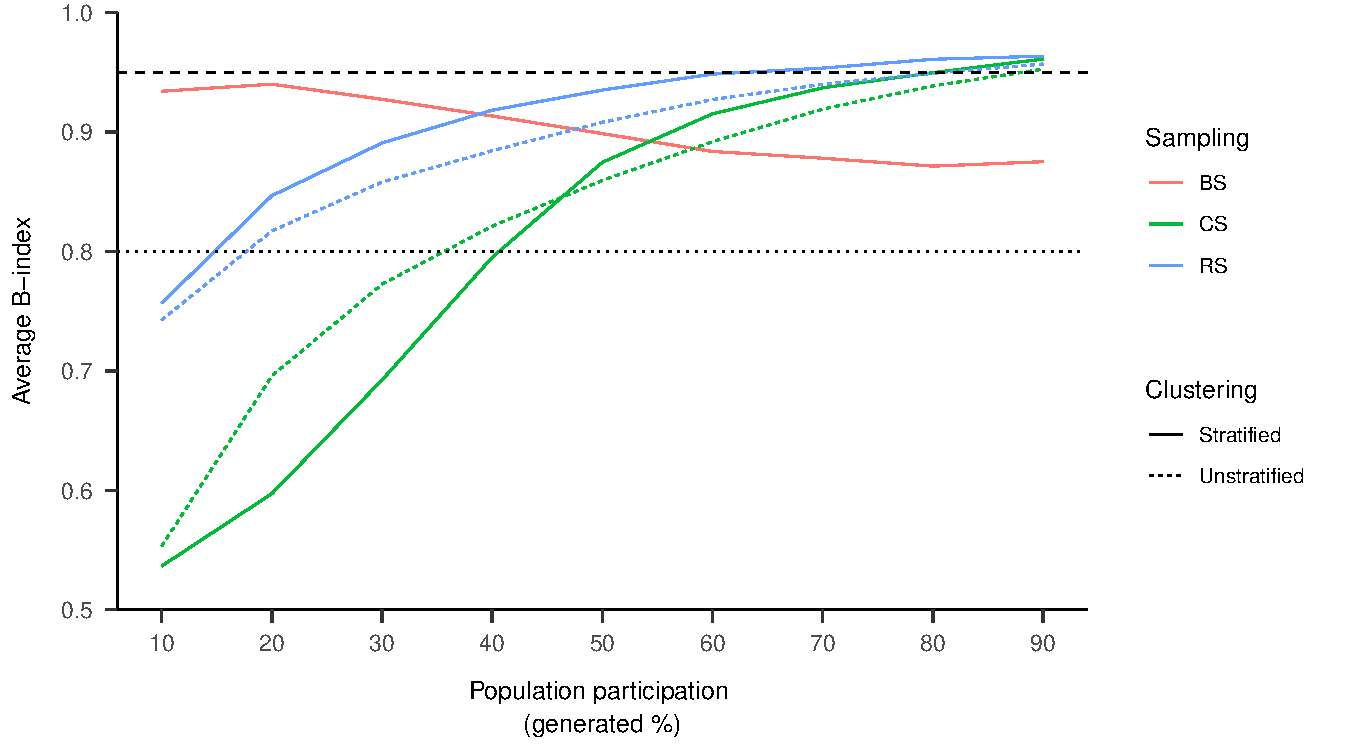
\includegraphics{6---Paper_files/figure-latex/fig-avg-B-1.pdf}
\caption{\label{fig:fig-avg-B}Average \(B\)-index for varying participation rates, by sampling method. Horizontal dotted line represented index of .95 indicating a high level of generalizability.}
\end{figure}

We also found several trends that were unexpected. At 50\% and beyond, SBS performance slowly degrades, while other methods maintain a steady increase. We expected a constant positive relationship between the population participation rate and the performance of all methods. Furthermore, at low response rates unstratified convenience sampling seemed to perform better than stratified convenience sampling. This seems counter-intuitive, as survey literature suggests that stratified samples are more representative. Because the B-index is an overall measure of generalizabilty across many covariates, it is difficult to untangle why these methods preformed as they did. We next examined the performance of the sampling methods on each individual covariate.

\hypertarget{standardized-mean-differences}{%
\subsubsection{Standardized Mean Differences}\label{standardized-mean-differences}}

We began this analysis by plotting mean SMDs for each covariate across all sampling methods against the population participation rate. Sampling methods were considered to perform well if they resulted in an average SMD value below .25 across iterations. The relative performance of the sampling methods were used to group covariates into four patterns of performance. The first group of covariates is displayed in figure \ref{fig:fig-SMD-group1}. For this set of covariates, stratified methods always resulted in better balance than non stratified methods, where all stratified methods resulted better balance than non stratified methods. Notably, SBS almost always outperformed all other mehtods.



\begin{figure}
\centering
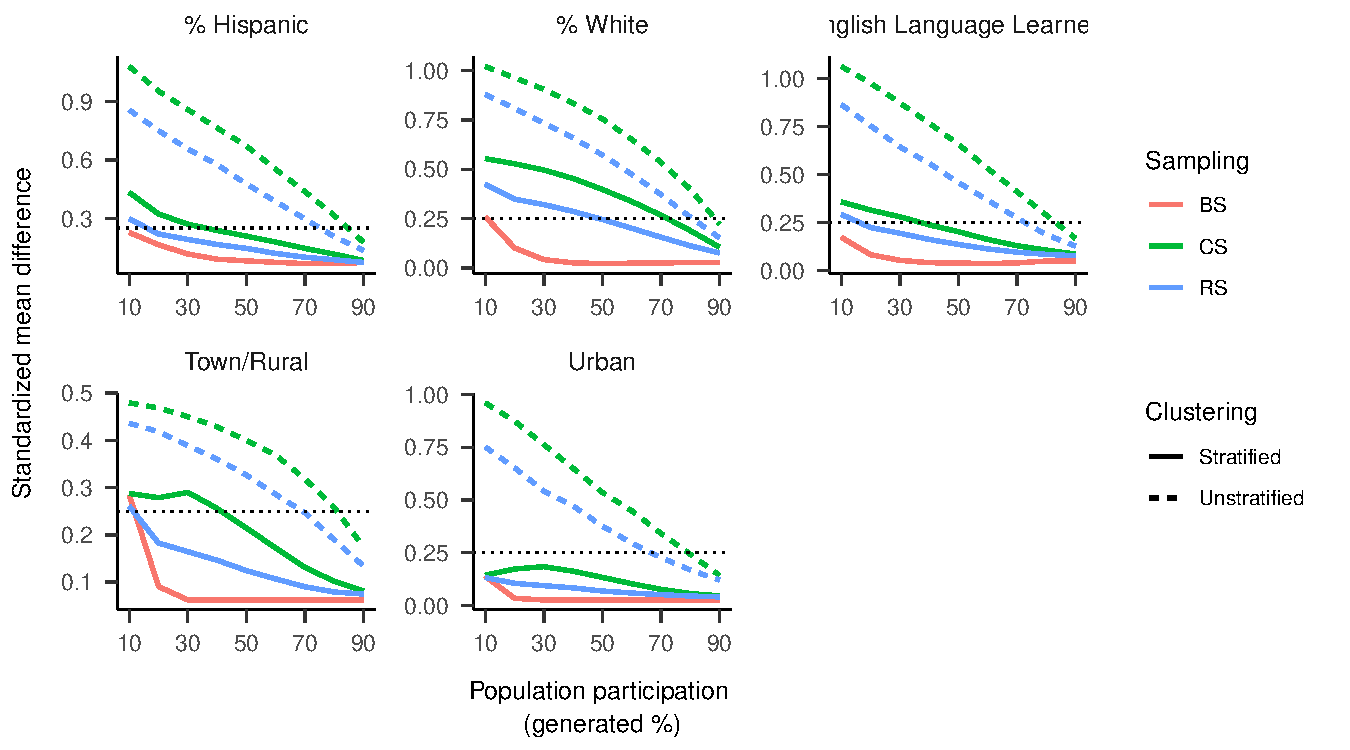
\includegraphics{6---Paper_files/figure-latex/fig-SMD-group1-1.pdf}
\caption{\label{fig:fig-SMD-group1}Group 1, good balance for stratified methods, poor balance for unstratified methods at low participation rates. Dotted horizontal line indicates a .25 cutoff.}
\end{figure}

The second group of covariates is displayed in figure \ref{fig:fig-SMD-group2}. Here, the stratified sampling methods consistently outperform their unstratified counterparts and almost always resulted in SMDs below .25. However, in some conditions, SCS performed worse than URS, or even SBS. Also, SBS was outperformed by SCS and SRS in certain conditions. The third group of covariates is displayed in figure \ref{fig:fig-SMD-group3}. Here, all sampling methods resulted in good balance across all population participation rates. SBS seemed to perform slightly better than all other methods, while differences between the other methods seems negligible. Finally, the fourth group of covariates is displayed in figure \ref{fig:fig-SMD-group4}. For these covariates, SBS performed consistently well across population participation rates. However, URS and UCS performed better than their stratified counterparts.



\begin{figure}
\centering
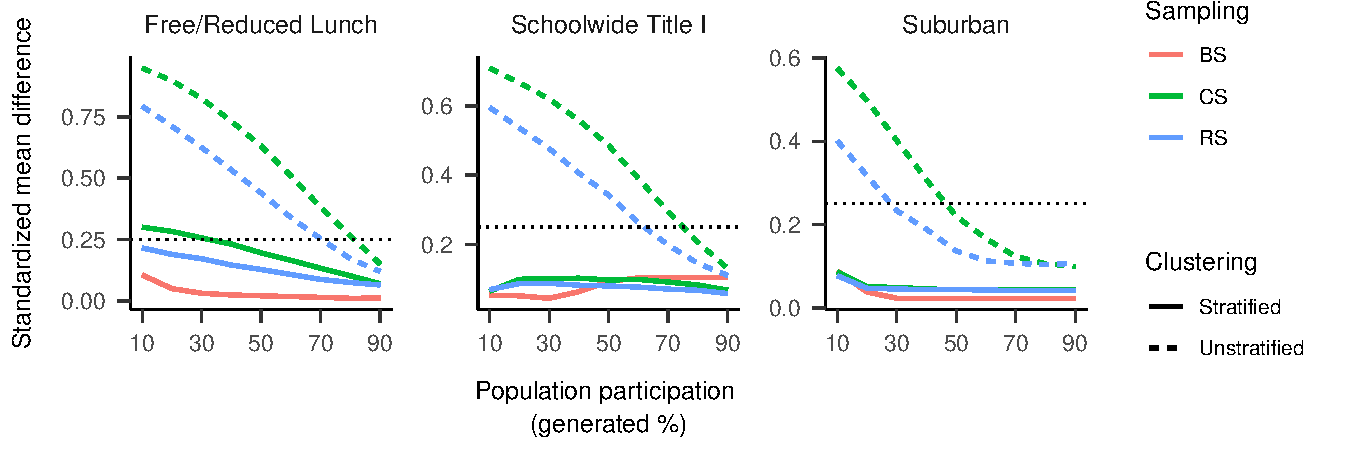
\includegraphics{6---Paper_files/figure-latex/fig-SMD-group2-1.pdf}
\caption{\label{fig:fig-SMD-group2}Group 2: good balance for stratified versions of methods, inconsistent performance by SBS and SCS. Dotted horizontal line indicates a .25 cutoff.}
\end{figure}



\begin{figure}
\centering
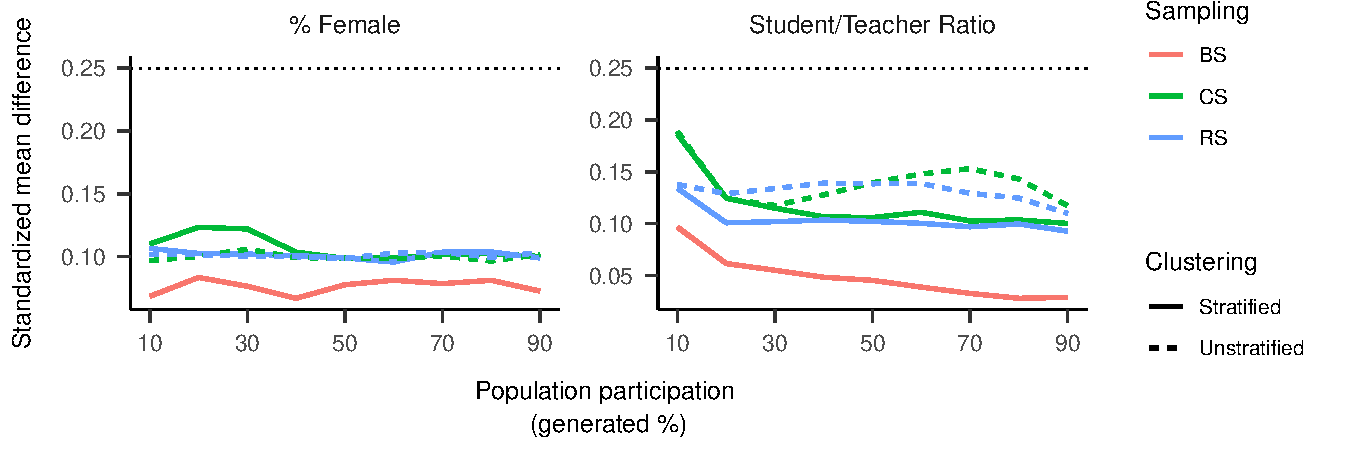
\includegraphics{6---Paper_files/figure-latex/fig-SMD-group3-1.pdf}
\caption{\label{fig:fig-SMD-group3}Group 3: all methods performed well, with SBS performing slightly better. Dotted horizontal line indicates a .25 cutoff.}
\end{figure}



\begin{figure}
\centering
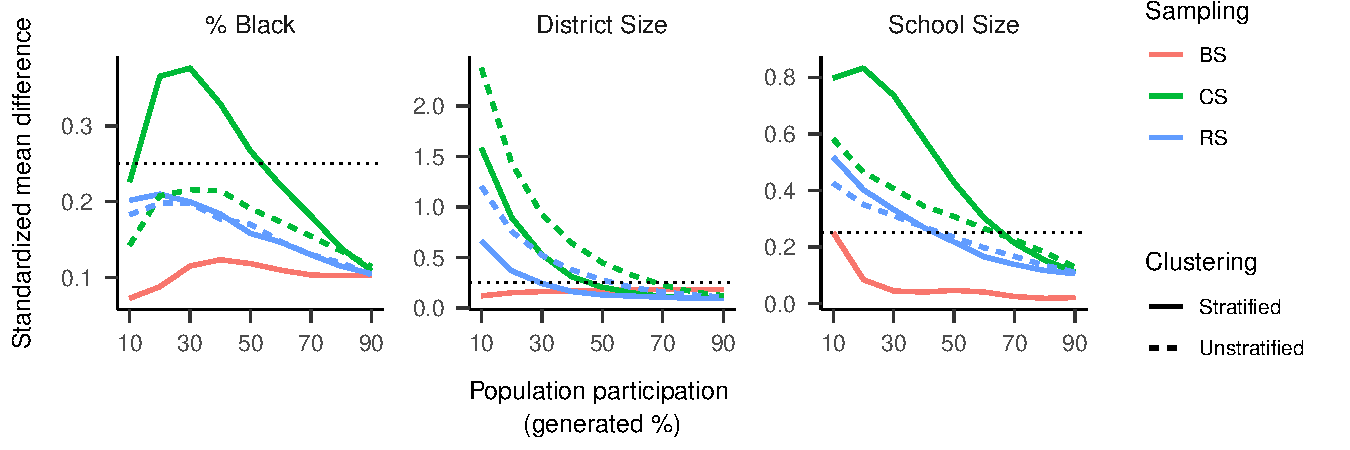
\includegraphics{6---Paper_files/figure-latex/fig-SMD-group4-1.pdf}
\caption{\label{fig:fig-SMD-group4}Group 4: poor relative performance for stratified convenience sampling and stratified random sampling. Dotted horizontal line indicates a .25 cutoff.}
\end{figure}

One potential explanation for why including stratification in a sampling design may result in poorer balance is that the strata are poorly specified. This may occur if the strata do not explain any variance in a covariate that is related to participation. To examine this we calculated the ICC for each covariate (i.e., the proportion of variance in the covariate that was between strata) and compared it to the log-odds coefficients associated with that covariate in the participation propensity model. We then plotted these values in figure \ref{fig:fig-Var-Coef}.

We noted several interesting relationships when examining the groups of covariate previously described,. Group 3, where all sampling methods performed well, consisted of covariates that were fairly unrelated to participation, and which played almost no role in generating strata. Group 4, where stratification seemed to reduce the performance of sampling methods, consisted of covariates that were predictive of participation, but were also overlooked by the strata generation process.



\begin{figure}
\centering
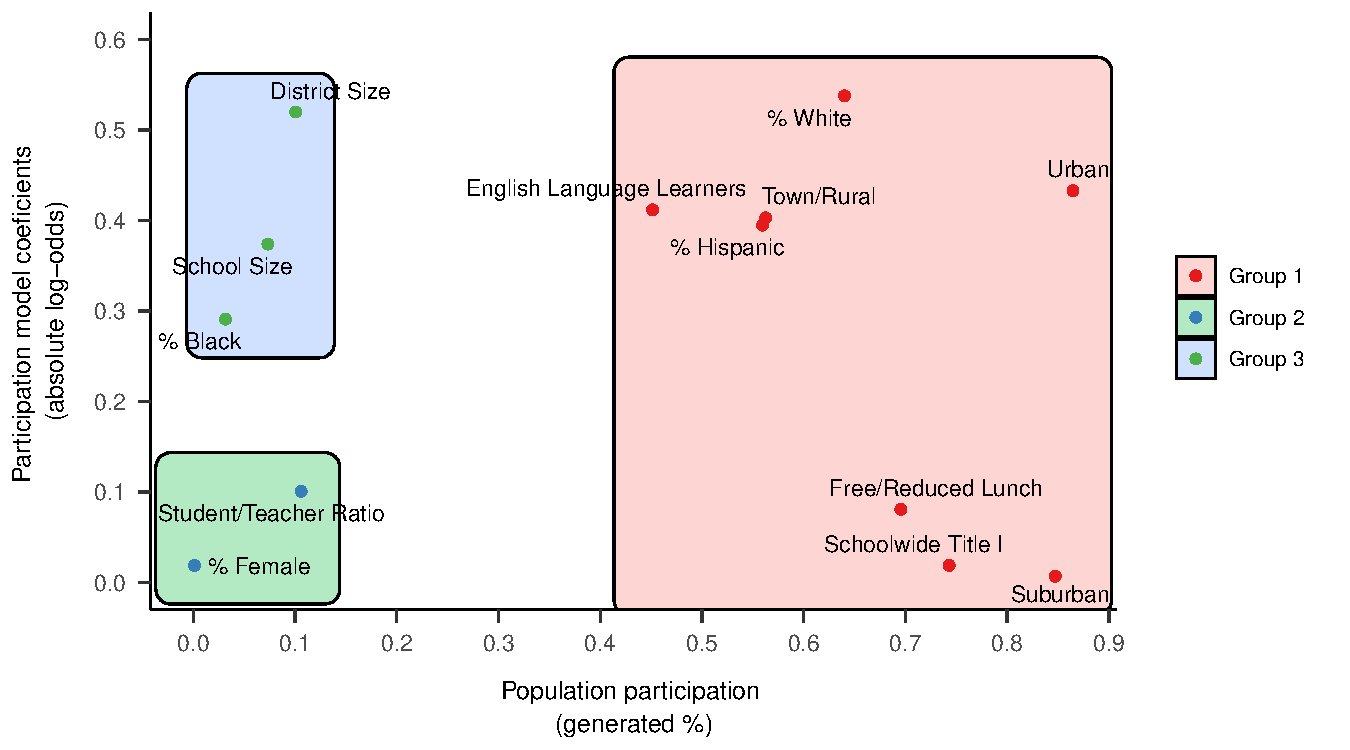
\includegraphics{6---Paper_files/figure-latex/fig-Var-Coef-1.pdf}
\caption{\label{fig:fig-Var-Coef}ICC Values vs absolute log odds. Shaded areas illustrate potential patterns in generalizability measured by SMDs.}
\end{figure}

\hypertarget{feasibility-1}{%
\subsection{Feasibility}\label{feasibility-1}}

\hypertarget{recruitment-attempts}{%
\subsubsection{Recruitment Attempts}\label{recruitment-attempts}}

Figure \ref{fig:fig-responses}a reports the total number of units that needed to be contacted to recruit a full sample of 60 schools across population participation rates for all sampling methods. Figure \ref{fig:fig-responses}b reports the percent of schools that agreed to participate across population participation rates for all sampling methods. Differences between sampling methods along these two measures were substantial at lower participation rates. As participation rates increased, the differences decreased exponentially and became negligible. It is important to note that the magnitudes of these results are quite extreme. This is likely due to some misspecification on the part of the simulation either in the response generating model parameters or the population participation rates. Rather than looking at the raw values, a more meaningful interpretation would be to compare the performance of the models relative to each other. Overall, UCS required the least \enquote{effort} to recruit a full sample, followed by URS and SCS, SRS, and finally SBS.



\begin{figure}
\centering
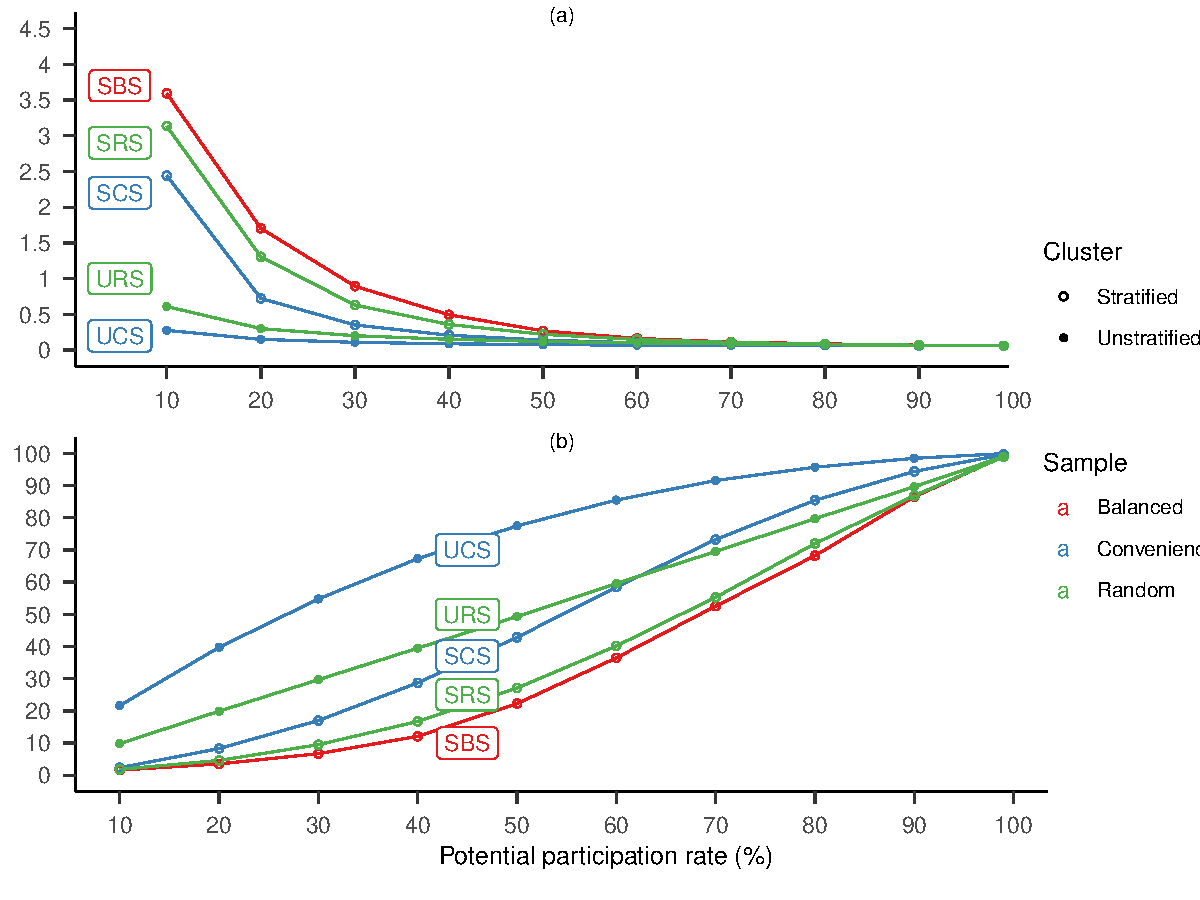
\includegraphics{6---Paper_files/figure-latex/fig-responses-1.pdf}
\caption{\label{fig:fig-responses}Sample recruitment statistics and response rates. Plot (a) shows the total number of units contacted to achieve a full sample of 60 schools. Plot (b) shows the percent of schools that agreed to participate when recruited.}
\end{figure}

\hypertarget{sampling-inequality-1}{%
\subsubsection{Sampling Inequality}\label{sampling-inequality-1}}

We calculated the Gini coefficient for each sampling method to examine the equality of sampling probabilities across methods. Figure \ref{fig:fig-gini} displays these for each sampling method across population participation rates. A coefficient of 1 indicates substantial sampling inequality. In the context of the simulation, a high Gini coefficient indicates that across iterations, only a small subset of the population was ever actually recruited.
Several trends emerged in this analysis. As population participation rates increased, inequality increased when using SBS, but decreased when using any other method. These four other methods also performed consistently relative to one another, with SRS resulting in the least amount of sampling inequality, followed by URS, SCS and UCS. As population rates increased, differences between stratified and unstratified versions of sampling methods seemed to decrease. This finding suggests that stratifying the population results in a larger potential sampling pool when the overall population response rate is low.



\begin{figure}
\centering
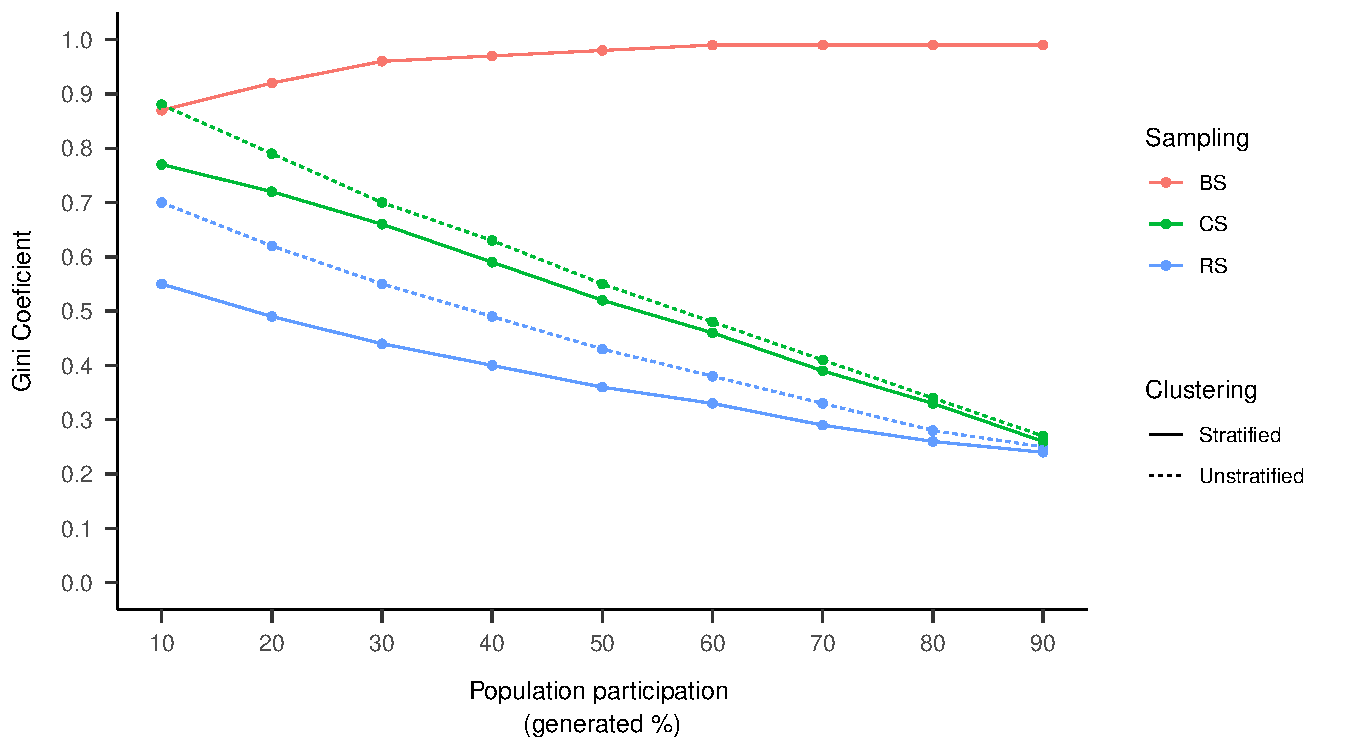
\includegraphics{6---Paper_files/figure-latex/fig-gini-1.pdf}
\caption{\label{fig:fig-gini}Gini coefficient across participation response rates for each sampling method. A coefficient of 1 indicates major inequality in sampling probability.}
\end{figure}

\hypertarget{summary-of-trends}{%
\subsection{Summary of Trends}\label{summary-of-trends}}

In terms of selecting a generalizable sample, SBS resulted in a considerable improvement compared to UCS. However, given the difficulty with which those samples are recruited, SBS is unlikely to be fully implemented in the ideal form. Instead, SCS may be a reasonable compromise. Our findings indicate that convenience and probability sampling methods are often improved by first stratifying the population. In certain cases, convenience sampling within strata (SCS) is comparable to simple random sampling (URS) both in terms of generalizability and feasibility.

An important observation which has not yet been addressed in the literature relates the specification of the clustering method to the response model. For instance, in Figure \ref{fig:fig-SMD-group4} we see that all methods of sampling result in balance on percentage of Black students, except for stratified convenience sampling. This is likely a result of the covariate having a strong relationship with participation, but not being weighed enough in the cluster analysis used in determining the strata. Figure \ref{fig:fig-Var-Coef} displays the calculated intraclass correlation coefficient (ICC) for each covariate along the strata, and the coefficient for each covariate in the response generating model. For covariates where one value (ICC or coefficient) is high, while the other is low, stratified sampling techniques resulted in poorer balance.

\hypertarget{discussion}{%
\section{Discussion}\label{discussion}}

The main goal of this study was to develop a framework for exploring the performance of sampling methods within the educational context. We put forth several models for algorithmically representing how researchers may select convenience sample of schools. Using prior work we also attempted to model how schools may decide whether or not to participate in a study if approached by recruiters. The methods we proposed for modeling these behaviors can, in principle, be extended to more complex and realistic specifications and adapted to other population frames.

A secondary goal was to use this framework in a demonstration of several sampling methods and their relative performance in terms of generalizability and feasibility. From this work we have drawn several conclusions. Stratified balanced sampling as proposed by Tipton (2013b) has the potential to greatly increase the generalizability of samples selected for MRTs. However, this method is not without limitations. Within our simulation, strict adherence came at a great cost in terms of sheer number of schools that needed to be contacted. Thus, implementing this method in practice may require allocating many more study resources to sample recruitment.

We found that ignoring the response model when specifying covariate weights during the cluster analysis stage may attenuate the generalizability of the resulting sample. Covariates that were not prioritized when generating the strata wound up being poorly represented in the final samples if they strongly predicted participation. Ignoring these relationships has the potential to undermine the investment of resources into SBS. Finally, while the balanced sampling approach does result in greater generalizability, it also appears to limit the actual pool of potential participants. Particularly in larger population response rates, the same subset of schools were likely to be recruited across iterations.

One potential compromise between current practice and SBS is to generate strata, but then implement convenience sampling within strata. As demonstrated in the simulations, stratified convenience sampling often resulted in better balance on individual covariates than simple random sampling. This may also elicit greater buy in from recruiters by placing less restrictions on what units they must sample.

Beyond generalizability, stratifying in this manner requires that researchers make sampling decisions in the study design phase, and to track changes in the sampling plan as recruitment progresses. Documenting and reporting this process would in turn support further research into developing more efficient and effective sampling methods.

\hypertarget{limitations}{%
\subsection{Limitations}\label{limitations}}

The models that we have studied make several key assumptions which represent limitations of the findings from the simulation study. First, in modeling convenience sampling, we assumed that recruiters always prioritize schools that are most likely to participate. In reality, other factors play a role as well, such as proximity of sample sites to the researcher and to each other, existing relationships between the recruiters and the sample sites, and other researcher assumptions about the sample site's characteristics. This limits how well our results reflect the performance of models in reality. Addressing this in future work can lead to better guidelines for future sampling designs.

Another implication of this assumption is that recruiters have approximate knowledge of how likely a sampled site is to participate. Though researchers may speculate about sites that are more willing to participate (such as schools in larger urban districts) and prioritize recruiting such sites, it is not likely that their estimation of \enquote{willingness} would be as close to the truth as we have estimated. Given this, it is possible that the \enquote{feasibility} of the convenience methods is over-stated, and that the degree of generalizability for some covariates is under-stated.

It is worth refining and exploring additional methods for modeling convenience sampling. The algorithms used in these methods can easily be tuned to include additional factors that might influence school recruitment priorities. For instance, location data is readily available and can therefore be incorporated into the model for how researchers prioritize schools in convenience sampling. Further work here could lead to more realistic and practical assessments of feasibility and generalizabilty, potentially providing researchers with a tool for evaluation sampling methods given their unique circumstances during the study design phase.

The second set of assumptions deals with the speculative nature of our participation model. In practice, the decision of whether a school participates in such a study often involves multiple stages. Generally, districts serve as gatekeepers, requiring submission and approval of research requests prior to recruitment. If the request is denied, no schools within the district may be recruited. If approved, researchers may work with a district-wide school coordinator, or may have to contact schools individually. In either cases, the ultimate decision may then rest with administrators, school research coordinators, or the teachers themselves.

A further limitation of the simulations is that the parameters in the response generating model are based on values from a study that examined the difference between schools participating in large-scale RCTs and the overall population of schools. However, these RCTs themselves typically rely on some form of convenience sampling. Consequently, our parameters reflect participation rates of schools that are likely to participate in RCTs, rather than the full population of schools. There simply isn't a solid understanding of what drives school participation in the current literature.

We believe that our findings reasonably represent the relative performance of the various sampling methods we tested in the context of educational research. However, a more exhaustive examination at what drives school participation in the population could address the above limitations and give us a better sense of how sampling methods would perform in reality. Disentangling participation bias from sampling bias requires researchers to implement probability based sampling or to be more transparent about their sampling practices. Doing so would also provide a deeper insight into school behavior and representation in research. If we can identify schools that are consistently and systematically under-represented in funded research, we can develop strategies to target such schools and increase the inclusivity of studies that strive for truly representative population level inferences.

\hypertarget{future-directions}{%
\subsection{Future Directions}\label{future-directions}}

This study has laid the groundwork for several avenues of research that are worth exploring further. First, additional work is needed on how best to optimize the cluster analysis. We have shown that the extent to which balance is achieved on a given covariate is related to how much that covariate drives strata generation and school participation. If some covariates are known to have greater influence on school participation, they should be weighted more heavily in generating the strata. Further work is also needed to understand the relationship between number of clusters generated, generalizability, and feasibility. It is expected that more clusters would increase generalizability, but also make recruitment more difficult. A better understanding of these relationships would help drive decision making during the design phase, which would make SBS much more accessible and quicker to initiate.

Further work also needs to examine the impact of these sampling methods on the bias and accuracy of population average treatment effect estimates. In this study, our goal was only to select a generalizable sample, where generalizability was operationalized as balance between the sample and population on a set of covariates. To the extent that the same covariates that dictate selection are also predictive of variance in treatment effects, we could extrapolate that a sample that is balanced on these covariates can be used to estimate an unbiased PATE. Reality is likely more complicated, however, and it would be worth examining the relationship between sampling and estimating unbiased treatment effects further.

Earlier we stated that if treatment effects are constant across units in a population, nonrandom samples of the population should still lead to unbiased estimates of average treatment effects. However, if only a narrow slice of the population is studied, there may not be enough variability in potential moderators to detect heterogeneity. Adding variation by selecting a more diverse sample may be useful if the presence of heterogeneity is unknown. This further complicates the specification of the cluster analysis. How should covariates be weighed relative to each other depending on whether they predict participation, differences in treatment effects, or some combination of both? To address this our work must be extended to study the relationship between sampling methods and bias in treatment effect estimation.

Large scale MRTs are expensive to implement, and resource allocation for such studies presents many difficult trade-offs. Researchers who wish to invest in robust recruitment strategies to amplify the impact and relevance of of their work should be better equipped to anticipate the costs and benefits of various sampling strategies. We hope that by showing the relative performance of these sampling methods, and by demonstrating the implementation of stratified sampling, we have contributed to future researchers being better informed in making these decisions.

\hypertarget{online-appendix}{%
\section{Online Appendix}\label{online-appendix}}

\hypertarget{sampling-feasibility}{%
\subsubsection{Sampling Feasibility}\label{sampling-feasibility}}

Figure \ref{fig:fig-rel-per} compares each sampling method to a reference method by plotting the factor of increased difficulty, calculated as the number of schools contacted by comparison method divided by the number of schools contacted by reference method. This gives us another perspective on the relative difficulty of each method. The straight horizontal line represents the reference method.



\begin{figure}
\centering
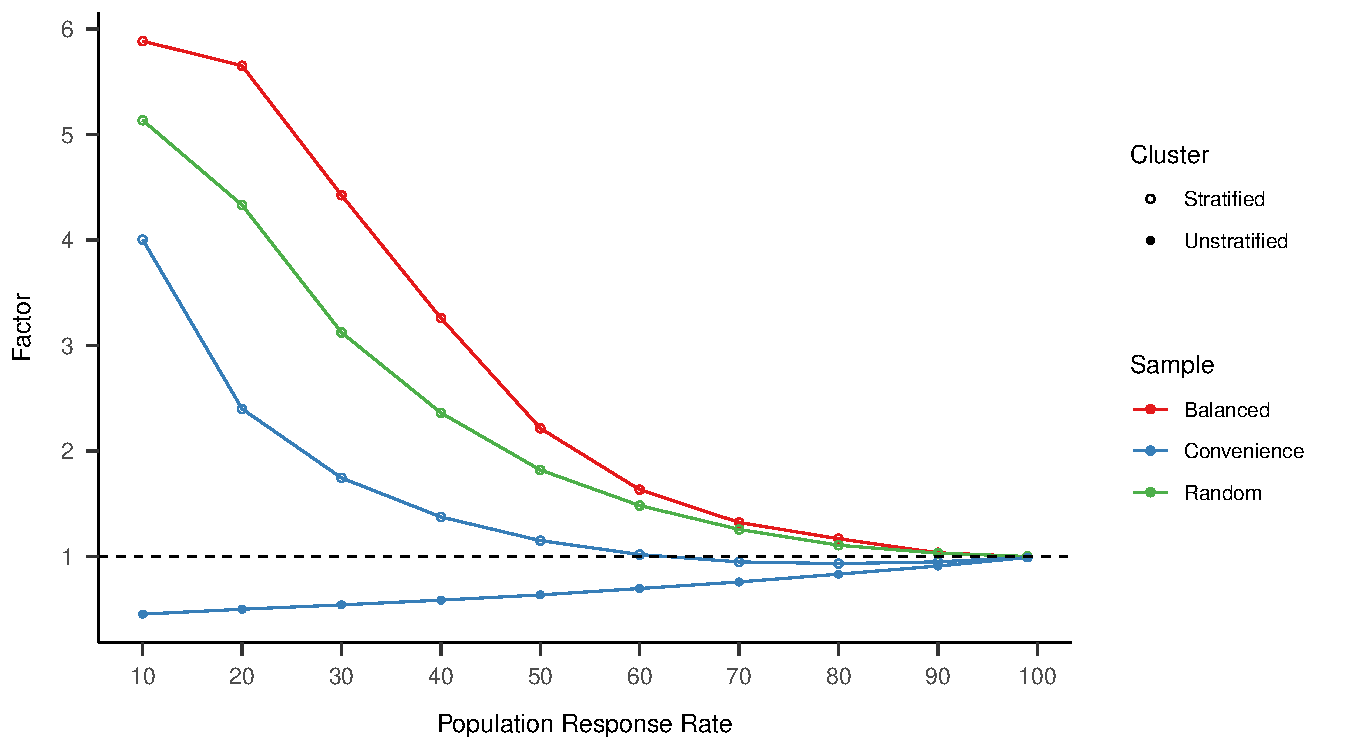
\includegraphics{6---Paper_files/figure-latex/fig-rel-per-1.pdf}
\caption{\label{fig:fig-rel-per}Relative sampling difficulty of each method compared to other methods. The straight horizontal line indicates the reference method being compared to.}
\end{figure}

\hypertarget{sampling-inequality-2}{%
\subsubsection{Sampling Inequality}\label{sampling-inequality-2}}

Figure \ref{fig:fig-gini-curve} displays the Gini curve and coefficient for all sampling methods across participation rates. The index is calculated by computing the area between the diagonal line and the curve. Coefficients of 0 indicate uniform equality across all sampling units, i.e.~all schools have an equal opportunity to be sampled. Coefficients of 1 indicate complete inequality, i.e.~very few schools are constantly being sampled across iterations. Overall, stratification results in lower inequality. However, since balanced sampling prioritizes schools according to set characteristics, the same schools are likely to be sampled each time.



\begin{sidewaysfigure}[p]
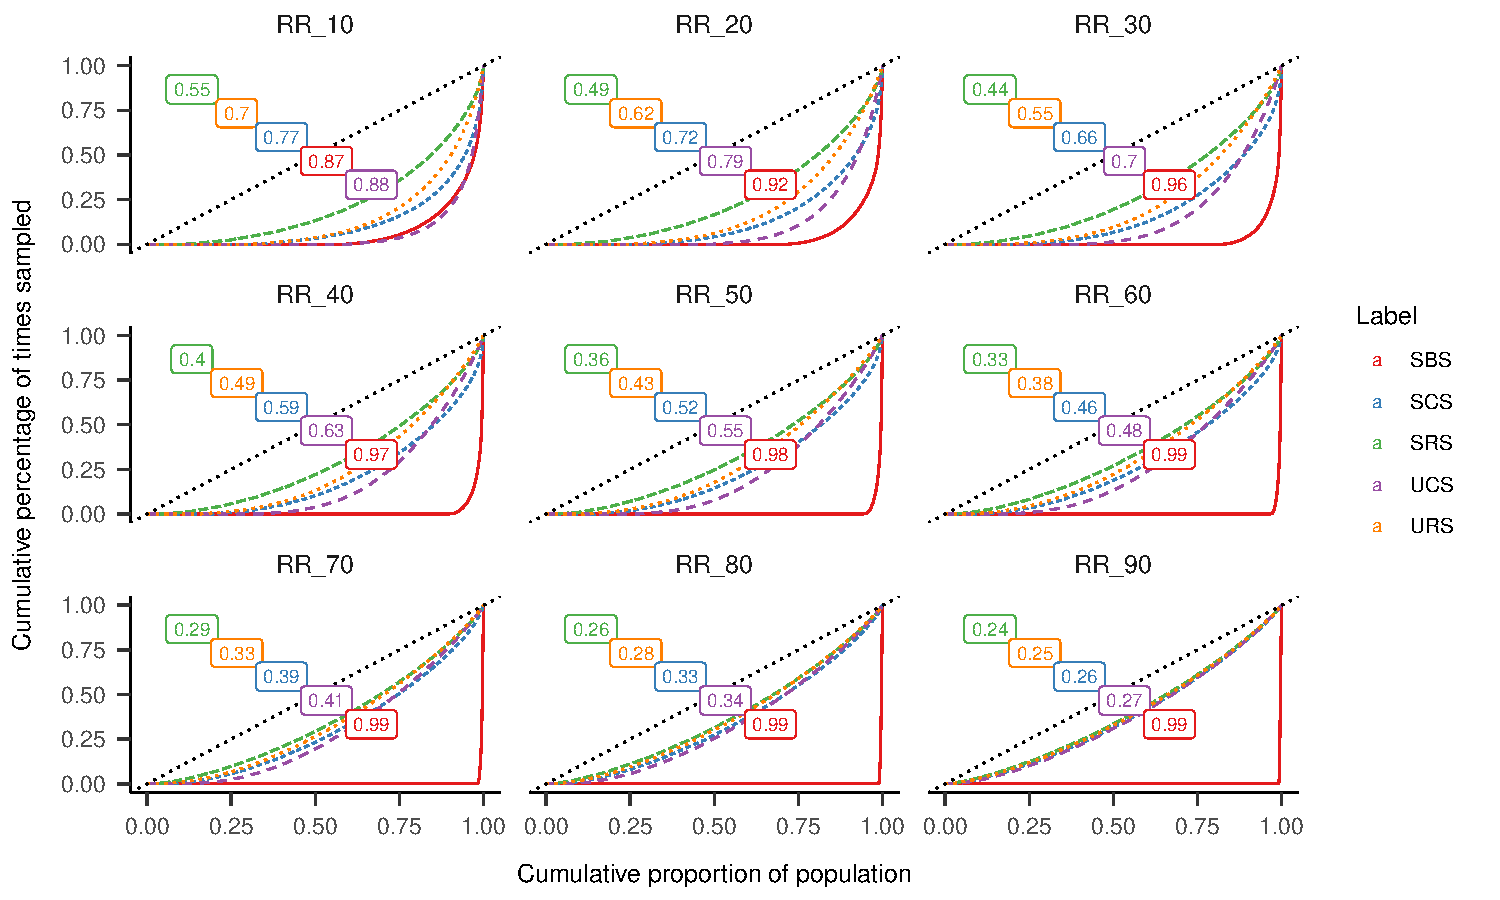
\includegraphics{6---Paper_files/figure-latex/fig-gini-curve-1} \caption{Cumulative probability plot and Gini coefficients representing the inequality of school sampling across sampling methods and population response rates.}\label{fig:fig-gini-curve}
\end{sidewaysfigure}

\newpage

\hypertarget{references}{%
\section{References}\label{references}}

\begingroup
\setlength{\parindent}{-0.5in}
\setlength{\leftskip}{0.5in}

\hypertarget{refs}{}
\leavevmode\hypertarget{ref-fellersDevelopingApproachDetermine2017}{}%
Fellers, L. (2017). \emph{Developing an approach to determine generalizability: A review of efficacy and effectiveness trials funded by the Institute of Education Sciences} (Ph.D.). Columbia University, United States -- New York. Retrieved from \url{https://search.proquest.com/docview/1865595768/abstract/40FD82F4A0C24535PQ/1}

\leavevmode\hypertarget{ref-gerberFieldExperimentsDesign2012}{}%
Gerber, A. S., \& Green, D. P. (2012). \emph{Field experiments: Design, analysis, and interpretation} (1st ed). New York: W. W. Norton.

\leavevmode\hypertarget{ref-grovesSurveyMethodology2004}{}%
Groves, R. M. (Ed.). (2004). \emph{Survey methodology}. Hoboken, N.J: Wiley-Interscience.

\leavevmode\hypertarget{ref-kernAssessingMethodsGeneralizing2016}{}%
Kern, H. L., Stuart, E. A., Hill, J., \& Green, D. P. (2016). Assessing Methods for Generalizing Experimental Impact Estimates to Target Populations. \emph{Journal of Research on Educational Effectiveness}, \emph{9}(1), 103--127. \url{https://doi.org/10.1080/19345747.2015.1060282}

\leavevmode\hypertarget{ref-olsenExternalValidityPolicy2013}{}%
Olsen, R. B., Orr, L. L., Bell, S. H., \& Stuart, E. A. (2013). External Validity in Policy Evaluations That Choose Sites Purposively. \emph{Journal of Policy Analysis and Management}, \emph{32}(1), 107--121. \url{https://doi.org/10.1002/pam.21660}

\leavevmode\hypertarget{ref-omuircheartaighGeneralizingUnrepresentativeExperiments2014}{}%
O'Muircheartaigh, C., \& Hedges, L. V. (2014). Generalizing from unrepresentative experiments: A stratified propensity score approach. \emph{Journal of the Royal Statistical Society: Series C (Applied Statistics)}, \emph{63}(2), 195--210. \url{https://doi.org/10.1111/rssc.12037}

\leavevmode\hypertarget{ref-raudenbush2015learning}{}%
Raudenbush, S. W., \& Bloom, H. S. (2015). Learning about and from a distribution of program impacts using multisite trials. \emph{American Journal of Evaluation}, \emph{36}(4), 475--499.

\leavevmode\hypertarget{ref-raudenbushStatisticalPowerOptimal2000}{}%
Raudenbush, S. W., \& Liu, X. (2000). Statistical power and optimal design for multisite randomized trials. \emph{Psychological Methods}, \emph{5}(2), 199--213. \url{https://doi.org/10.1037//1082-989X.5.2.199}

\leavevmode\hypertarget{ref-shadishExperimentalQuasiexperimentalDesigns2002}{}%
Shadish, W. R., Cook, T. D., \& Campbell, D. T. (2002). \emph{Experimental and quasi-experimental designs for generalized causal inference}. Boston, MA, US: Houghton, Mifflin and Company.

\leavevmode\hypertarget{ref-stuartCharacteristicsSchoolDistricts2017}{}%
Stuart, E. A., Bell, S. H., Ebnesajjad, C., Olsen, R. B., \& Orr, L. L. (2017). Characteristics of School Districts That Participate in Rigorous National Educational Evaluations. \emph{Journal of Research on Educational Effectiveness}, \emph{10}(1), 168--206. \url{https://doi.org/10.1080/19345747.2016.1205160}

\leavevmode\hypertarget{ref-stuartUsePropensityScores2011}{}%
Stuart, E. A., Cole, S. R., Bradshaw, C. P., \& Leaf, P. J. (2011). The use of propensity scores to assess the generalizability of results from randomized trials: Use of Propensity Scores to Assess Generalizability. \emph{Journal of the Royal Statistical Society: Series A (Statistics in Society)}, \emph{174}(2), 369--386. \url{https://doi.org/10.1111/j.1467-985X.2010.00673.x}

\leavevmode\hypertarget{ref-tiptonImprovingGeneralizationsExperiments2013}{}%
Tipton, E. (2013a). Improving Generalizations From Experiments Using Propensity Score Subclassification: Assumptions, Properties, and Contexts. \emph{Journal of Educational and Behavioral Statistics}, \emph{38}(3), 239--266. Retrieved from \url{https://www.jstor.org/stable/41999424}

\leavevmode\hypertarget{ref-tiptonStratifiedSamplingUsing2013}{}%
Tipton, E. (2013b). Stratified Sampling Using Cluster Analysis: A Sample Selection Strategy for Improved Generalizations From Experiments. \emph{Evaluation Review}, \emph{37}(2), 109--139. \url{https://doi.org/10.1177/0193841X13516324}

\leavevmode\hypertarget{ref-tiptonHowGeneralizableYour2014}{}%
Tipton, E. (2014). How Generalizable Is Your Experiment? An Index for Comparing Experimental Samples and Populations. \emph{Journal of Educational and Behavioral Statistics}, \emph{39}(6), 478--501.

\leavevmode\hypertarget{ref-tiptonSiteSelectionExperiments2016}{}%
Tipton, E., Fellers, L., Caverly, S., Vaden-Kiernan, M., Borman, G., Sullivan, K., \& de Castilla, V. R. (2016). Site Selection in Experiments: An Assessment of Site Recruitment and Generalizability in Two Scale-up Studies. \emph{Journal of Research on Educational Effectiveness}, \emph{9}(sup1), 209--228. \url{https://doi.org/10.1080/19345747.2015.1105895}

\leavevmode\hypertarget{ref-tiptonImplicationsSmallSamples2017}{}%
Tipton, E., Hallberg, K., Hedges, L. V., \& Chan, W. (2017). Implications of Small Samples for Generalization: Adjustments and Rules of Thumb. \emph{Evaluation Review}, \emph{41}(5), 472--505. \url{https://doi.org/10.1177/0193841X16655665}

\leavevmode\hypertarget{ref-tiptonImprovedGeneralizabilityImproved2019}{}%
Tipton, E., \& Matlen, B. J. (2019). Improved Generalizability Through Improved Recruitment: Lessons Learned From a Large-Scale Randomized Trial. \emph{American Journal of Evaluation}, \emph{40}(3), 414--430. \url{https://doi.org/10.1177/1098214018810519}

\leavevmode\hypertarget{ref-tipton2020toward}{}%
Tipton, E., Spybrook, J., Fitzgerald, K. G., Wang, Q., \& Davidson, C. (2020). Toward a system of evidence for all: Current practices and future opportunities in 37 randomized trials. \emph{Educational Researcher}, 0013189X20960686.

\endgroup


\end{document}
